\documentclass[11pt]{article}
\usepackage[T1,T2A]{fontenc}
\usepackage[utf8]{inputenc}
\usepackage[english,russian]{babel}
\usepackage{graphicx}
\graphicspath {{img/}}
\title{\textbf{Лабораторная работа №1\\<<Знакомство с системой автоматизированного проектирования Multisim for education>>}}
\author{Матяш А.А., ККСО-01-19}
\date{}
\addtolength{\topmargin}{-3cm}
\addtolength{\textheight}{3cm}
\begin{document}
\maketitle
\thispagestyle{empty}
\textbf{Цель работы:} научиться использовать возможности программы Multisim для изучения свойств сетей и систем передачи информации и приобретение практических навыков
\section{Перечень элементов на схемах}
\subsection{<<Амплитудный демодулятор>>}
\begin{itemize}
    \item[-] Источник переменного тока (220 В, 50 Гц)
    \item[-] Диод
    \item[-] Конденсатор (1 мФ)
    \item[-] Резистор (10 Ом)
    \item[-] Ключ
    \item[-] Четырех канальный осциллограф
    \item[-] Вольтметр
\end{itemize}
\subsection{<<Интегрирующая RC-цепь>>}
\begin{itemize}
    \item[-] Источник переменного тока (5 В, 2 кГц)
    \item[-] Резистор (1 кОм)
    \item[-] Конденсатор (1 мкФ)
    \item[-] Четырех канальный осциллограф
    \item[-] Построитель частотных характеристик
\end{itemize}
\subsection{<<Генератор слов - логический анализатор>>}
\begin{itemize}
    \item[-] Логический анализатор (16 канальный)
    \item[-] Генератор слов (32 канальный)
    \item[-] Индикаторы 8 шт. (2.5 В)
\end{itemize}
\subsection{<<Логические элементы>>}
\begin{itemize}
    \item[-] Цифровой источник питания (5 В)
    \item[-] Ключи 4 шт.
    \item[-] Логическое НЕ
    \item[-] Логическое И (3)
    \item[-] Логическое ИЛИ (2)
    \item[-] Логическое Исключающее ИЛИ (3)
    \item[-] Индикатор (2.5 В)
    \item[-] Шестнадцатиричный дисплей
\end{itemize}
\subsection{<<Исследование АЦП и ЦАП>>}
\begin{itemize}
    \item[-] Функциональный генератор
    \item[-] Четырех канальный осциллограф
    \item[-] АЦП
    \item[-] ЦАП
    \item[-] Источник постоянного тока 2 шт. (5 В)
    \item[-] Источник тактового напряжения (5 В, 5000 Гц)
\end{itemize}
\subsection{<<Исследование спектра сигналов>>}
\begin{itemize}
    \item[-] Источник переменного тока (120 В, 30 кГЦ)
    \item[-] Источник переменного тока (240 В, 60 кГЦ)
    \item[-] Сумматор напряжения
    \item[-] Ключ
    \item[-] Спектральный анализатор
\end{itemize}
\section{Копии окон схемных файлов с позиционными обозначениями}
\subsection{<<Амплитудый демодулятор>>}
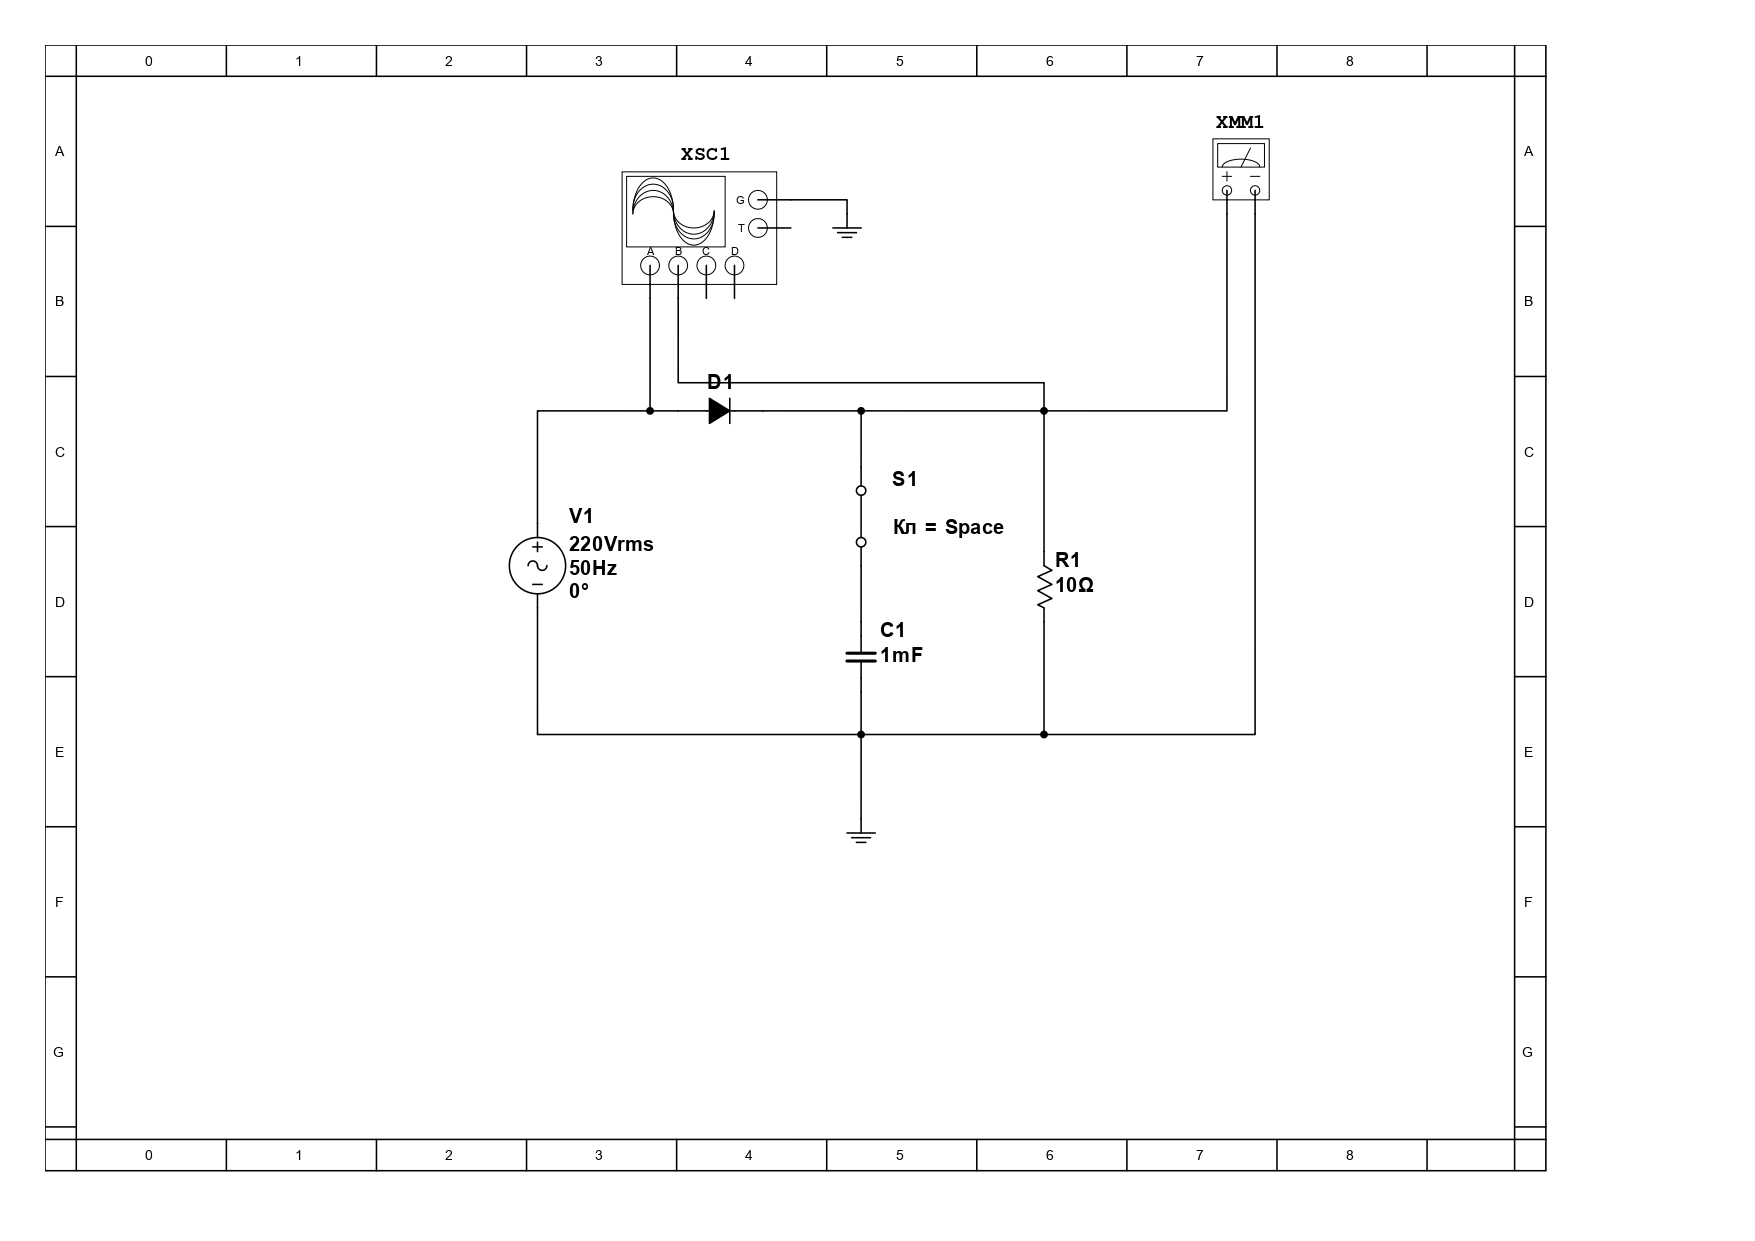
\includegraphics[width=1\linewidth]{1/scheme.jpg}
\subsection{<<Интегрирующая RC-цепь>>}
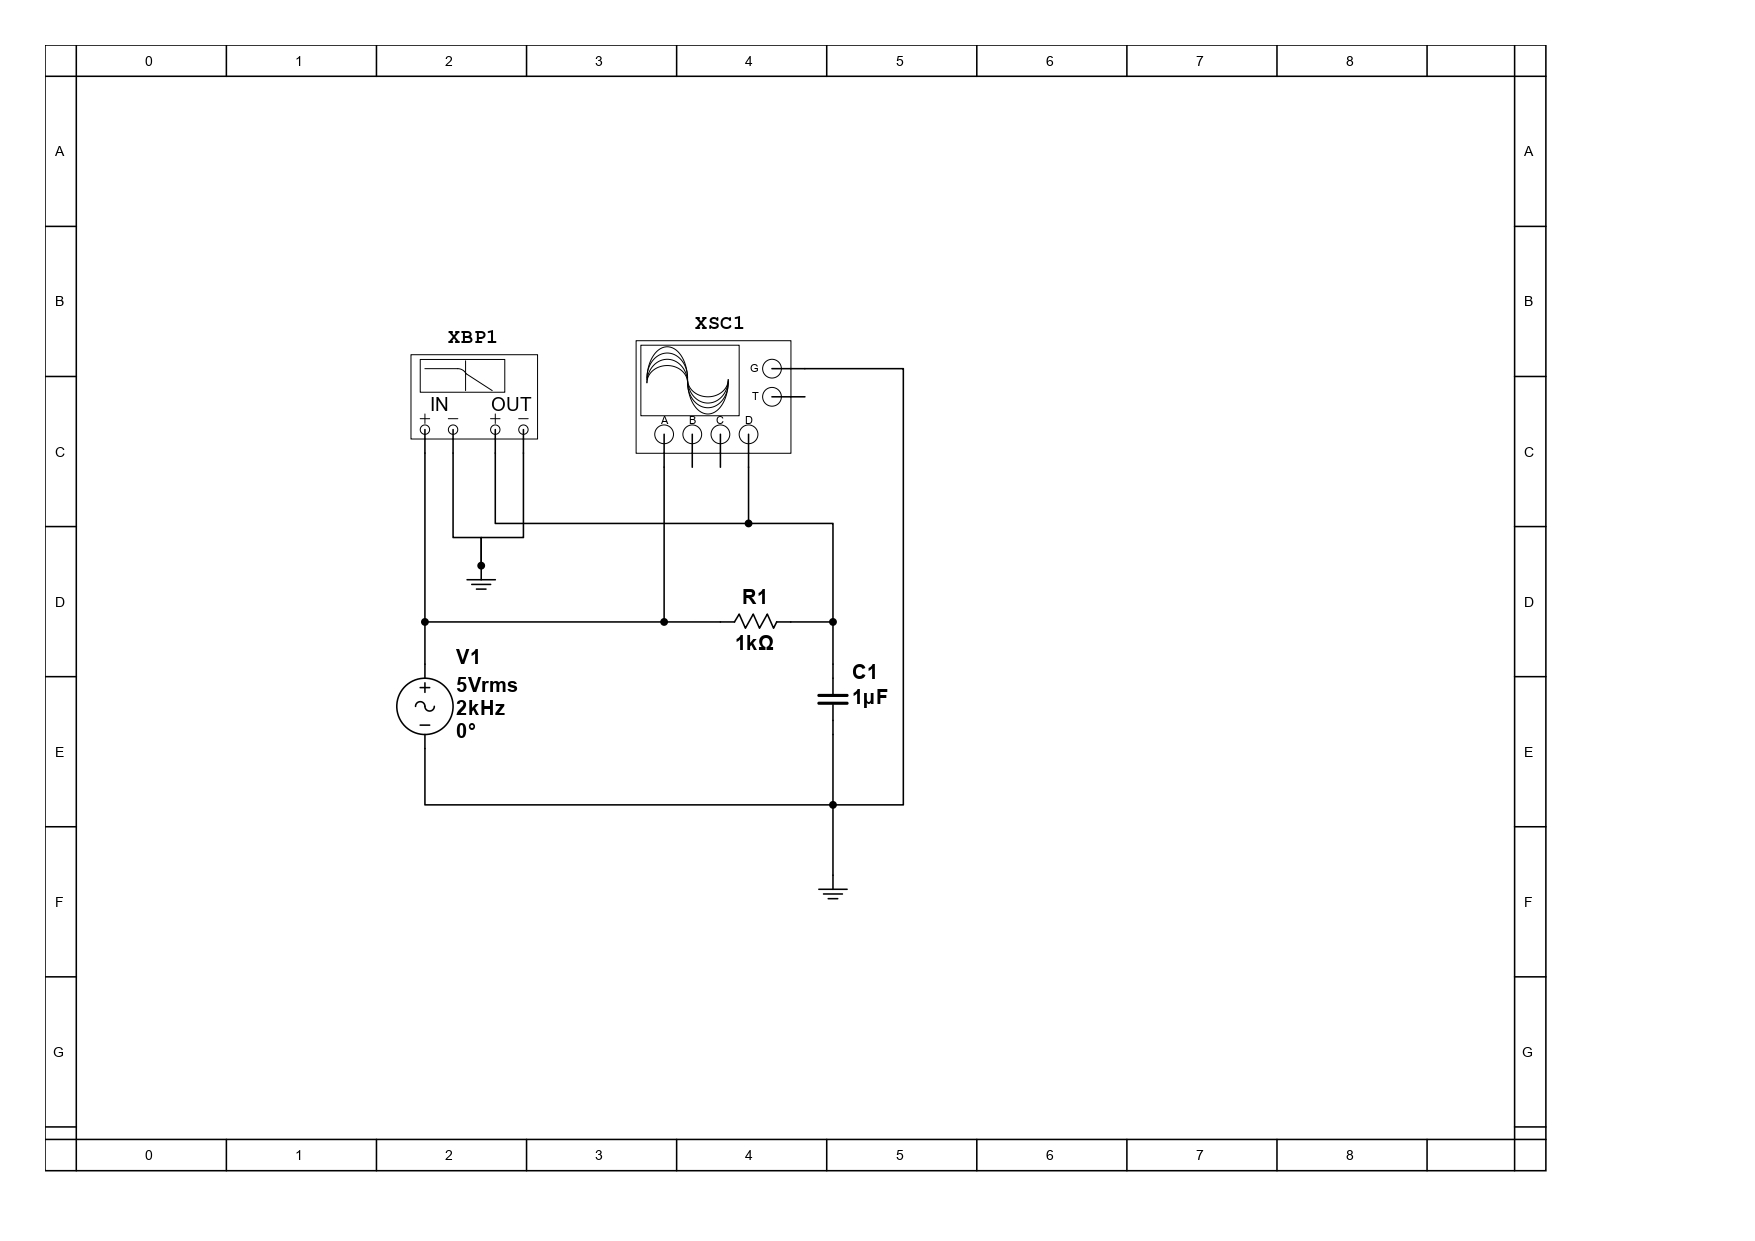
\includegraphics[width=1\linewidth]{2/scheme.jpg}
\subsection{<<Генератор слов - логический анализатор>>}
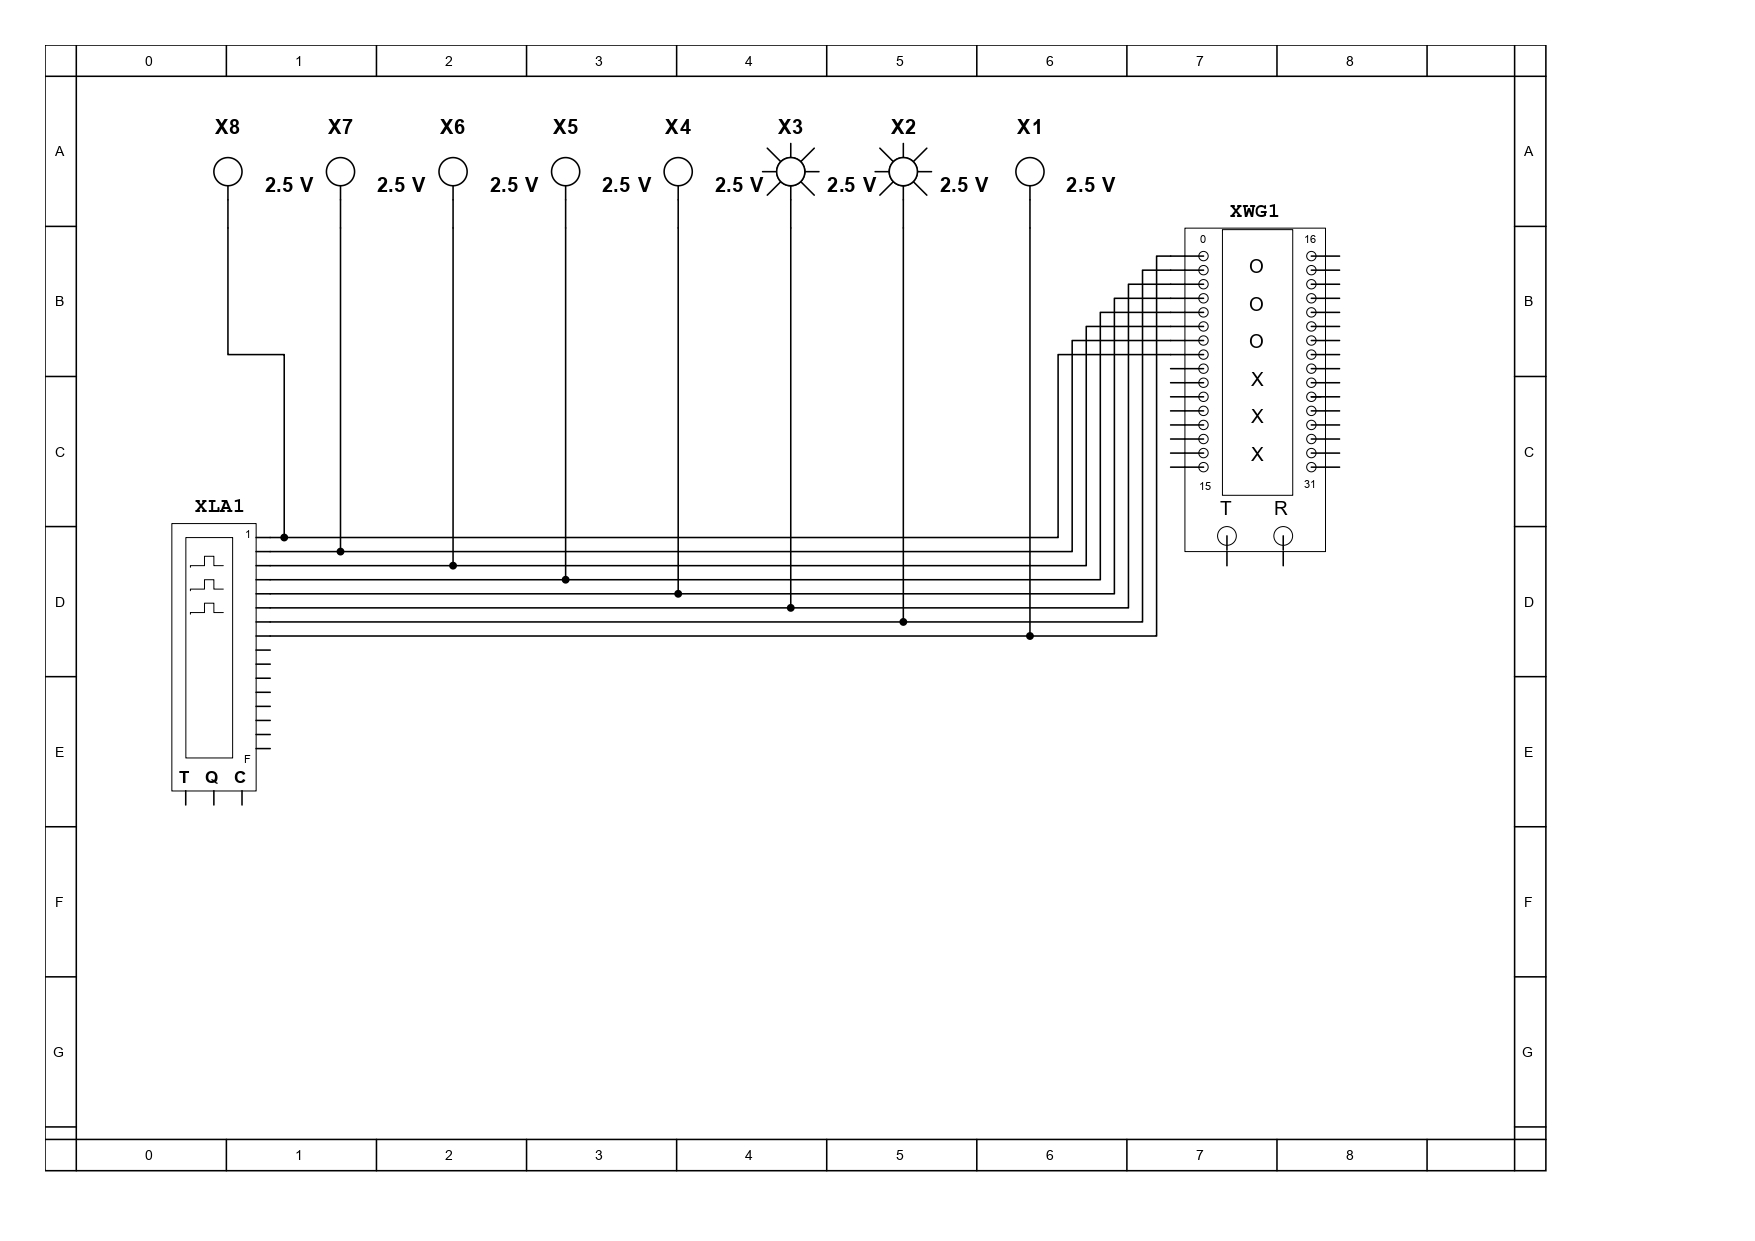
\includegraphics[width=1\linewidth]{3/scheme.jpg}
\subsection{<<Логические элементы>>}
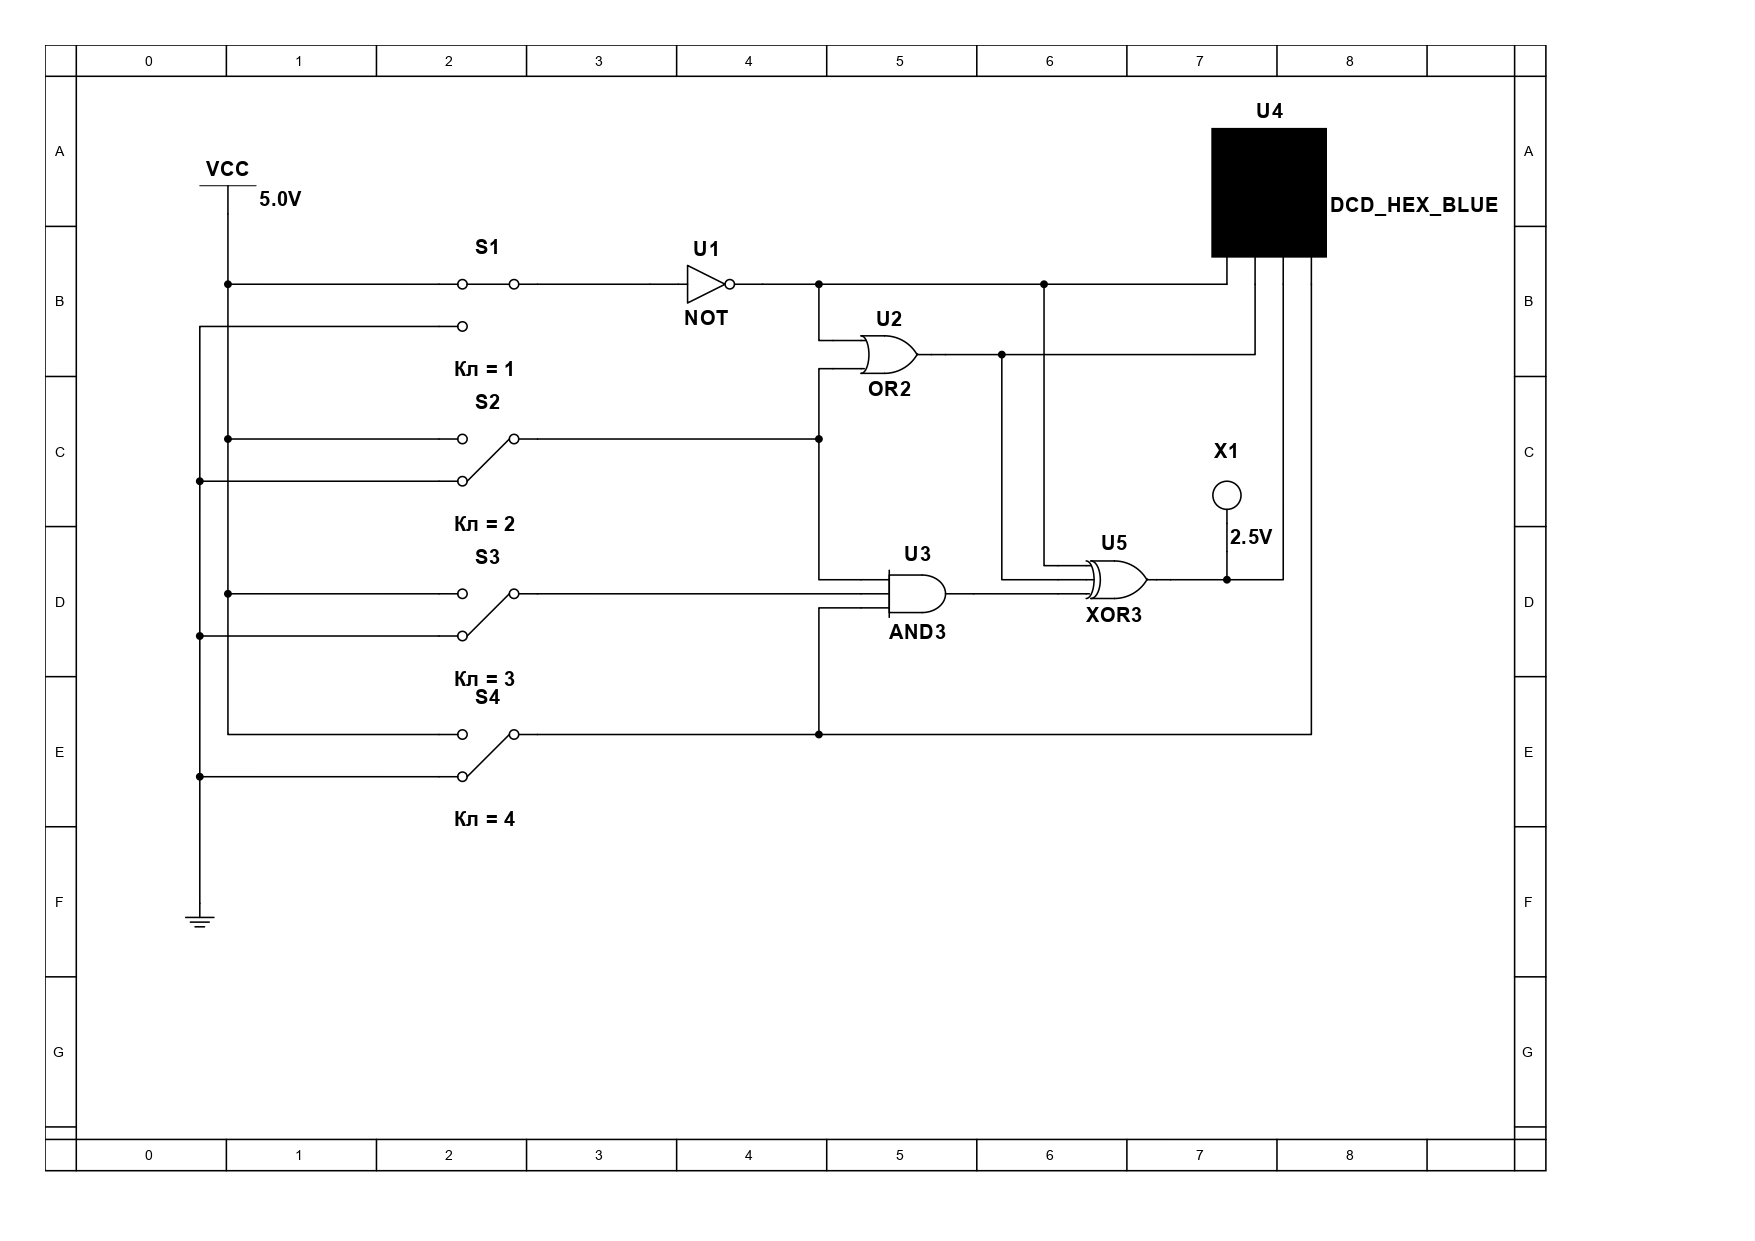
\includegraphics[width=1\linewidth]{4/scheme.jpg}
\subsection{<<Исследование АЦП и ЦАП>>}
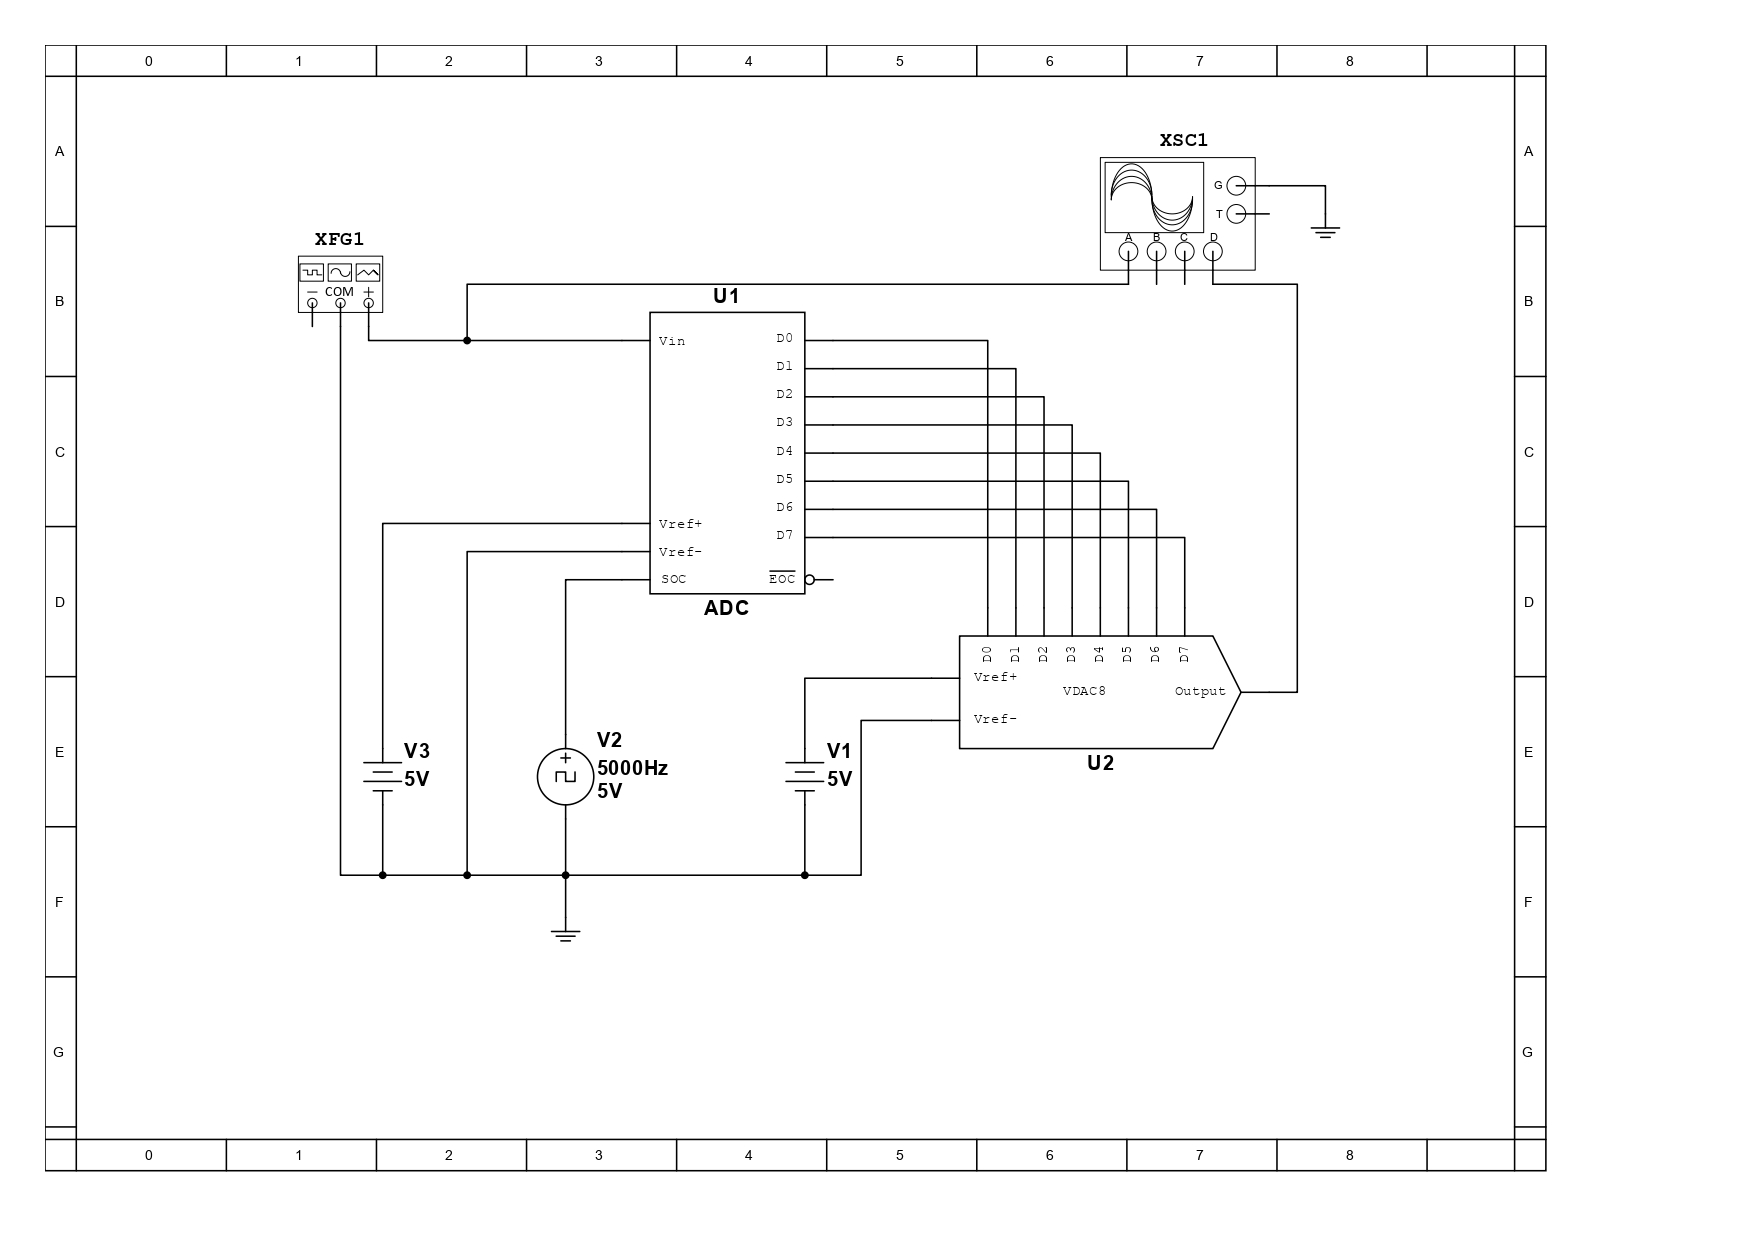
\includegraphics[width=1\linewidth]{5/scheme.jpg}
\subsection{<<Исследование спектра сигналов>>}
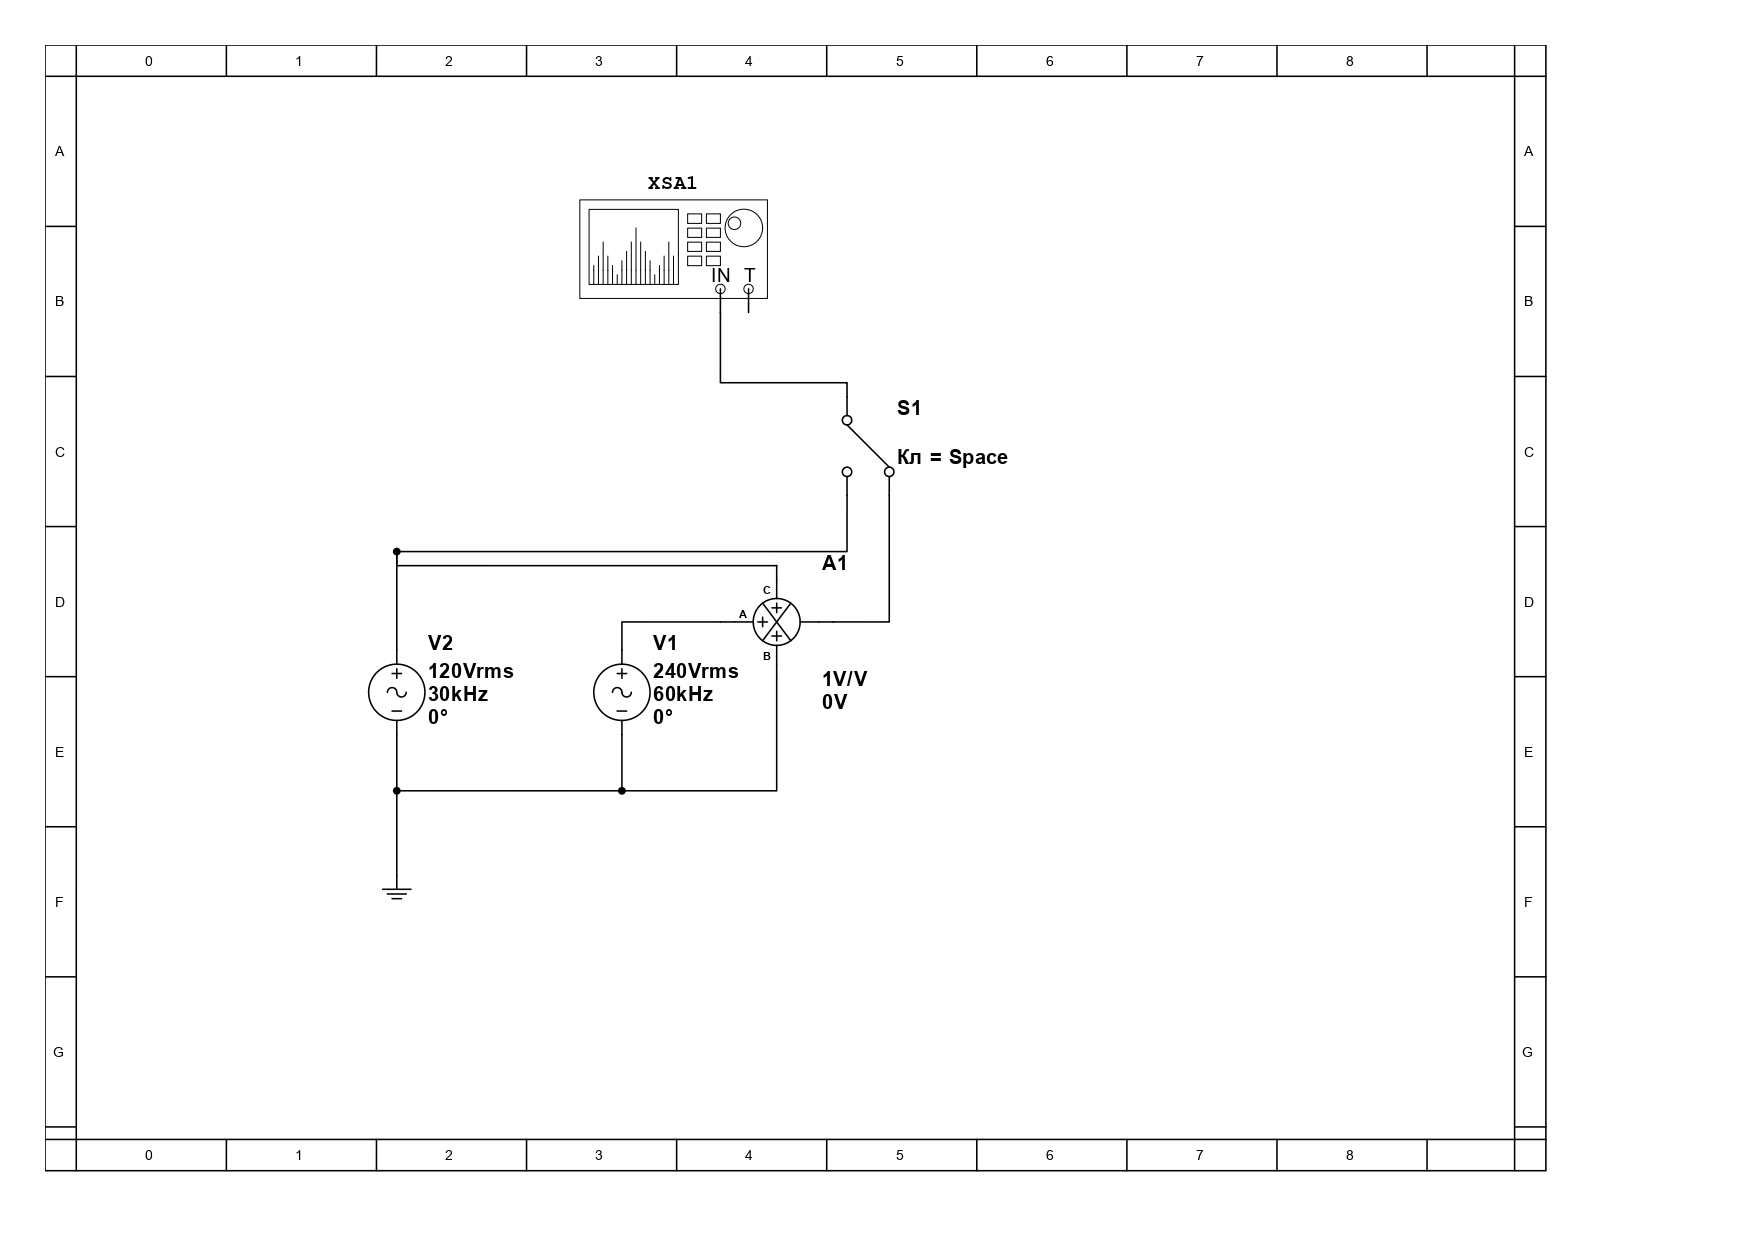
\includegraphics[width=1\linewidth]{6/scheme.jpg}
\section{<<Результаты измерений приборами>>}
\subsection{<<Амплитудый демодулятор>>}
Осцилограммы:
\begin{center}
    Ключ открыт
    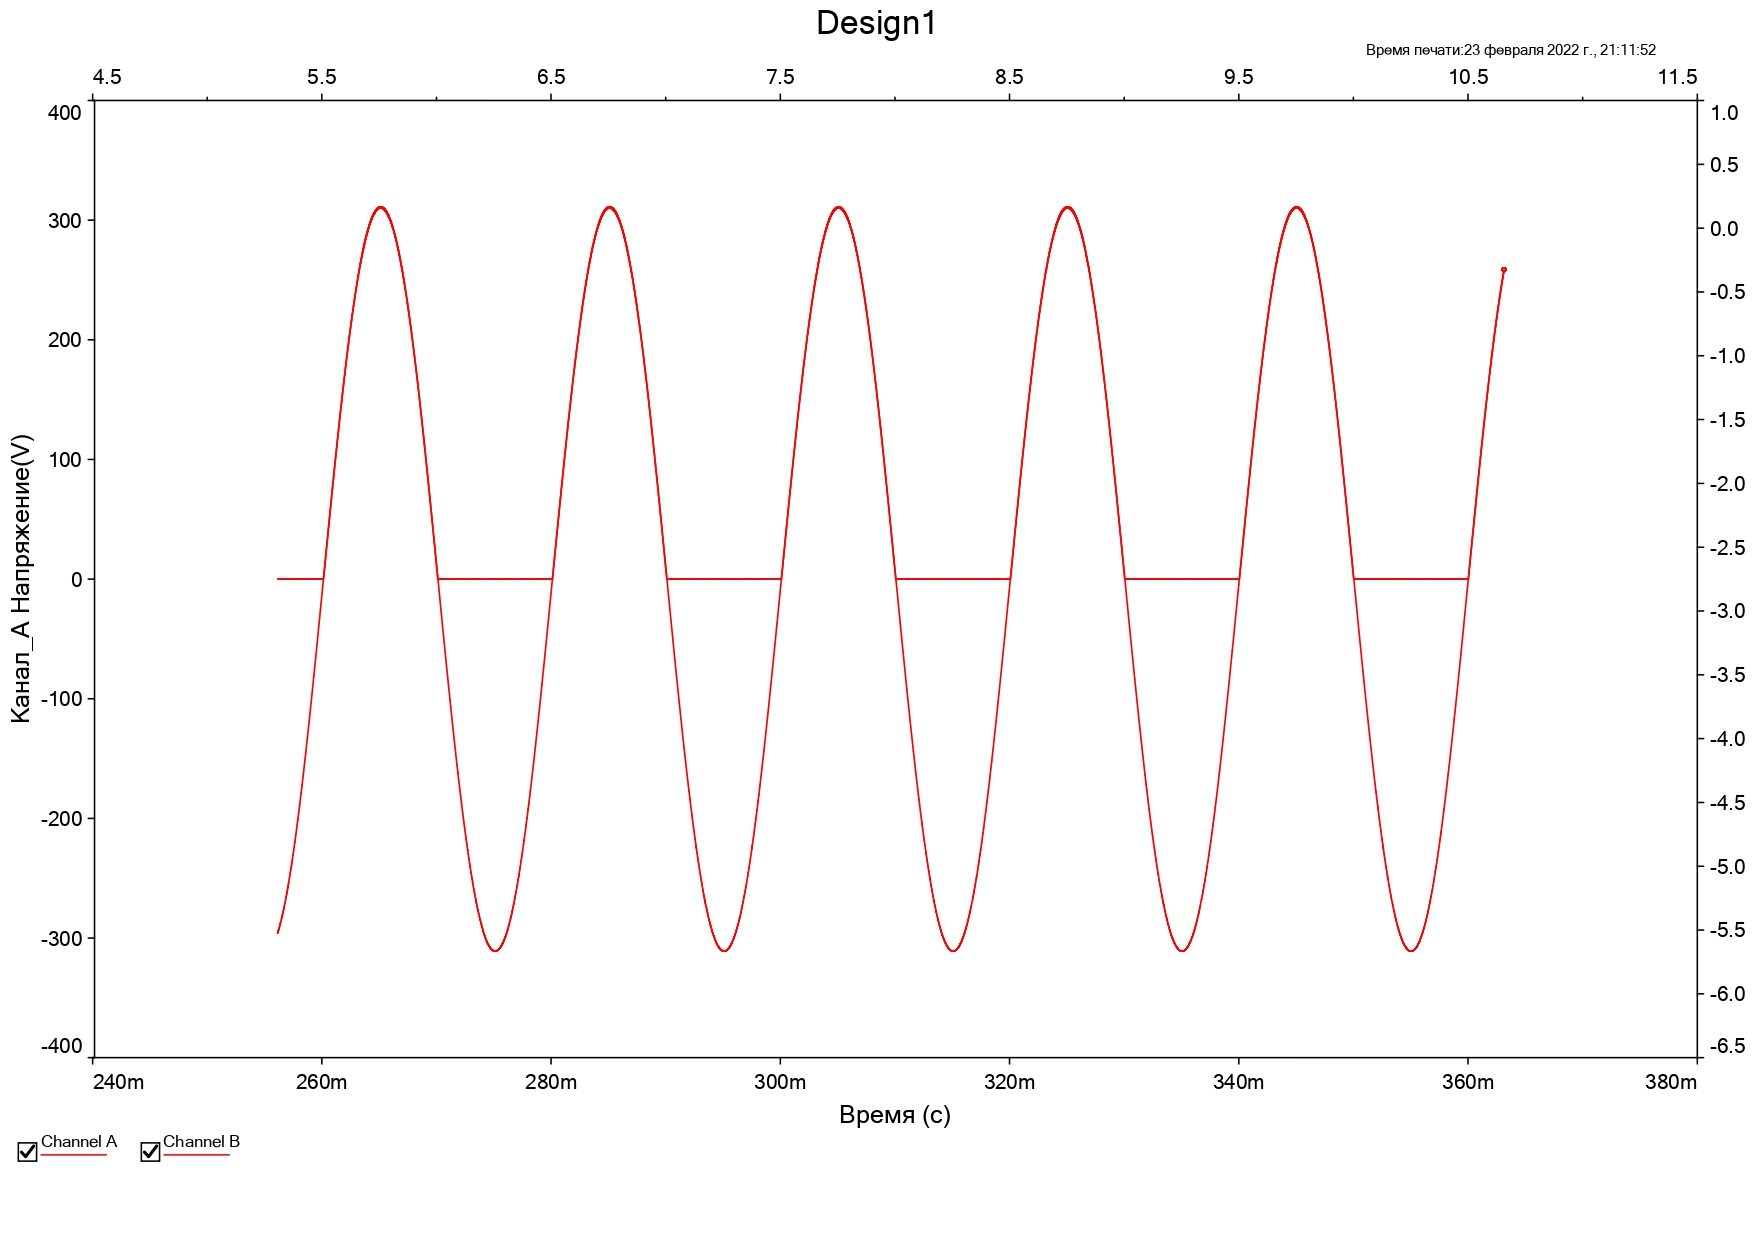
\includegraphics[width=1\linewidth]{1/osc_key_open.jpg}
\end{center}
Показания вольтметра: 98.56 В
\begin{center}
    Ключ закрыт
    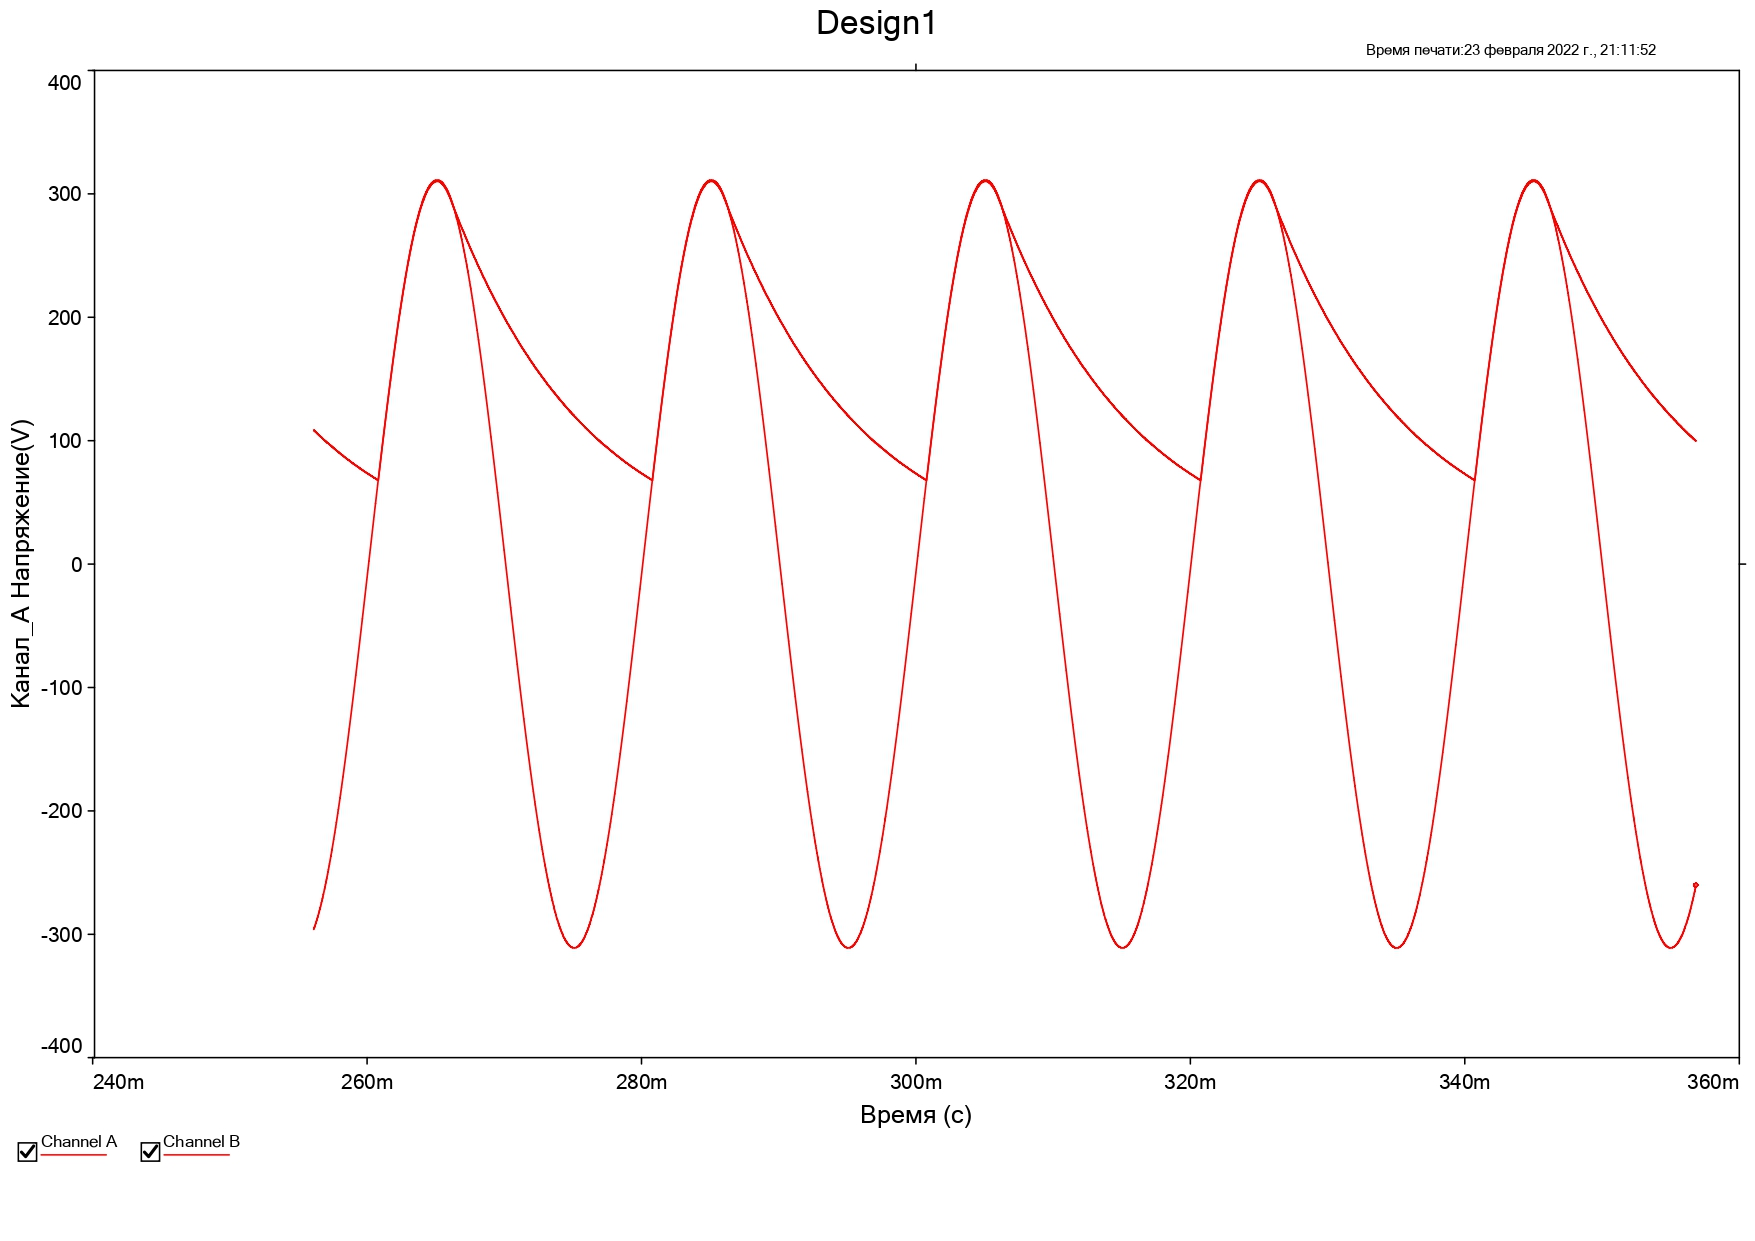
\includegraphics[width=1\linewidth]{1/osc_key_close.jpg}
\end{center}
Показания вольтметра: 176.98 В
\subsection{<<Интегрирующая RC-цепь>>}
\begin{center}
    Частотные характеристики
    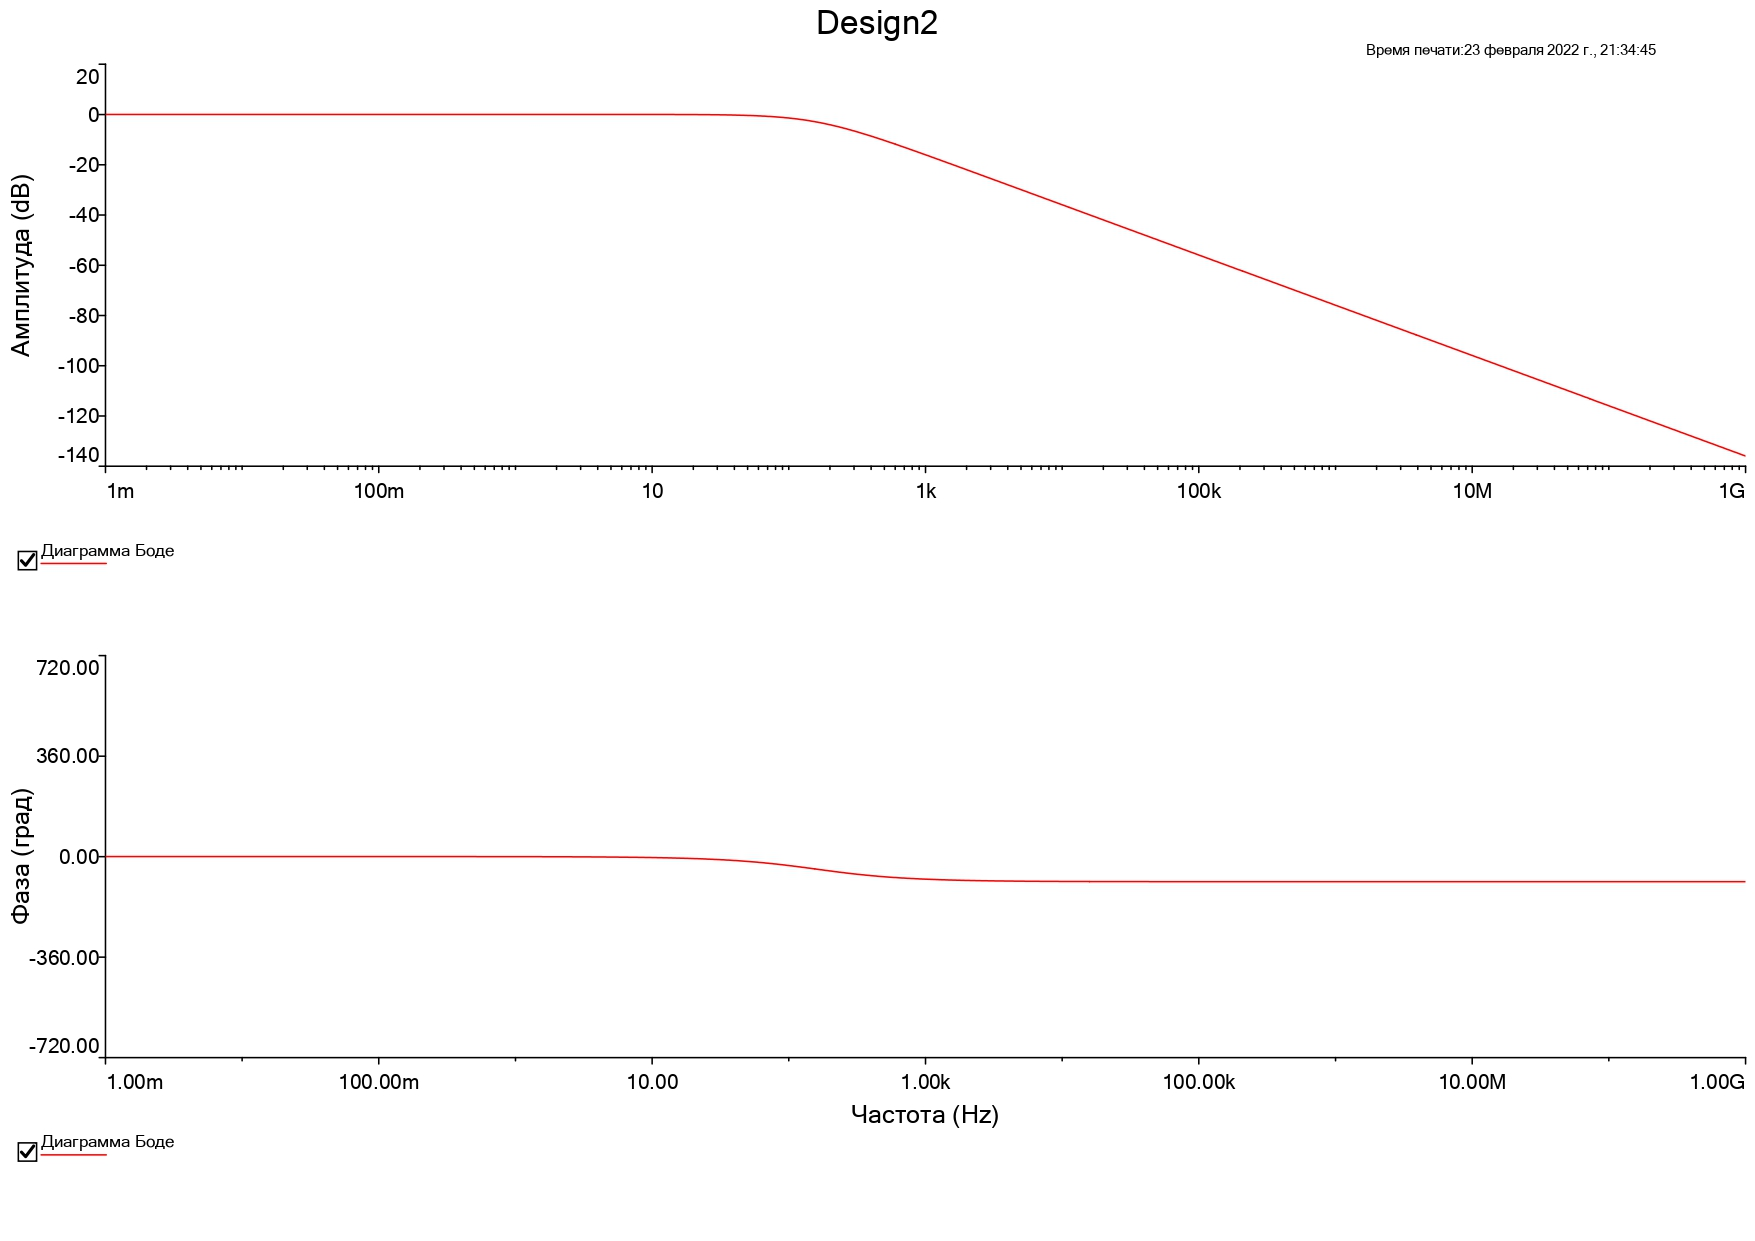
\includegraphics[width=1\linewidth]{2/gra1.jpg}
    Осцилограмма
    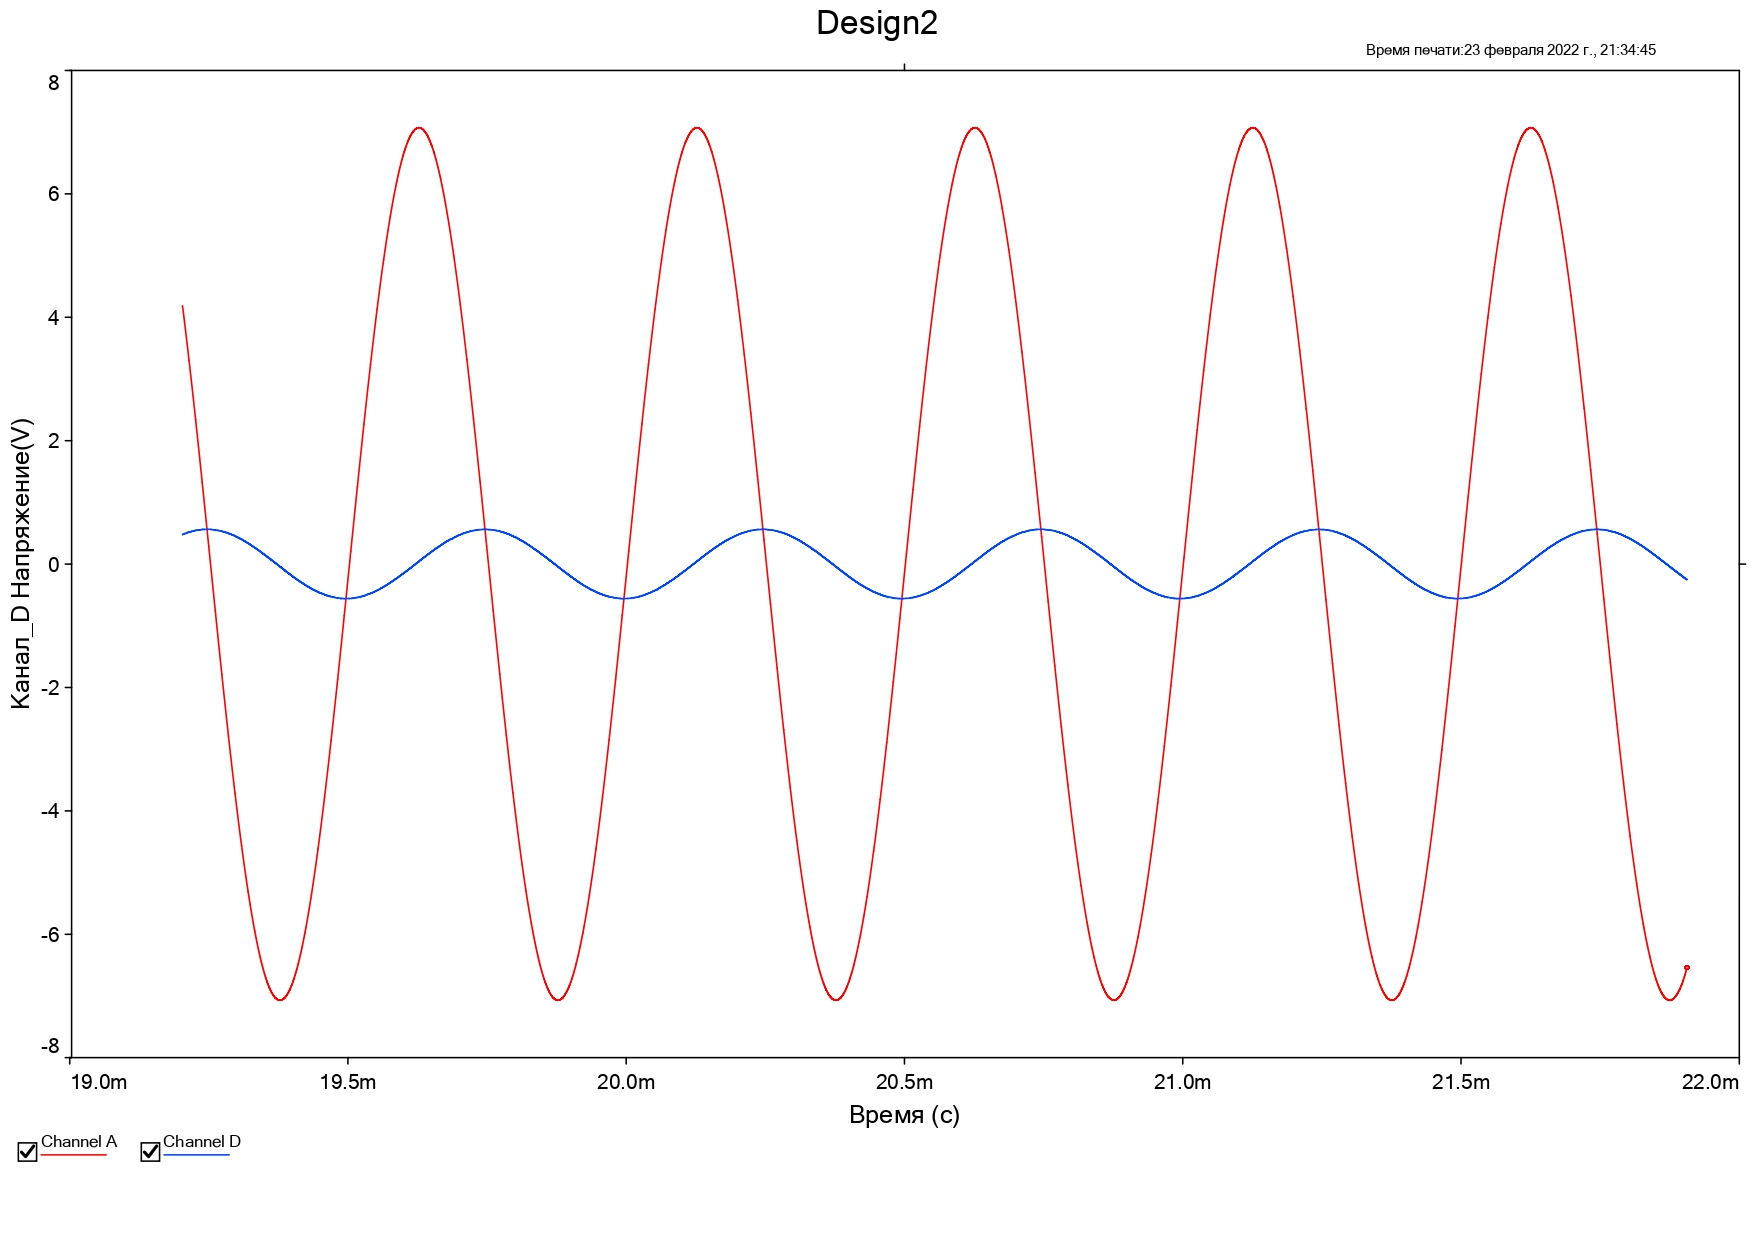
\includegraphics[width=1\linewidth]{2/gra2.jpg}
\end{center}
\subsection{<<Генератор слов - логический анализатор>>}
\begin{center}
    Показания логического анализатора
    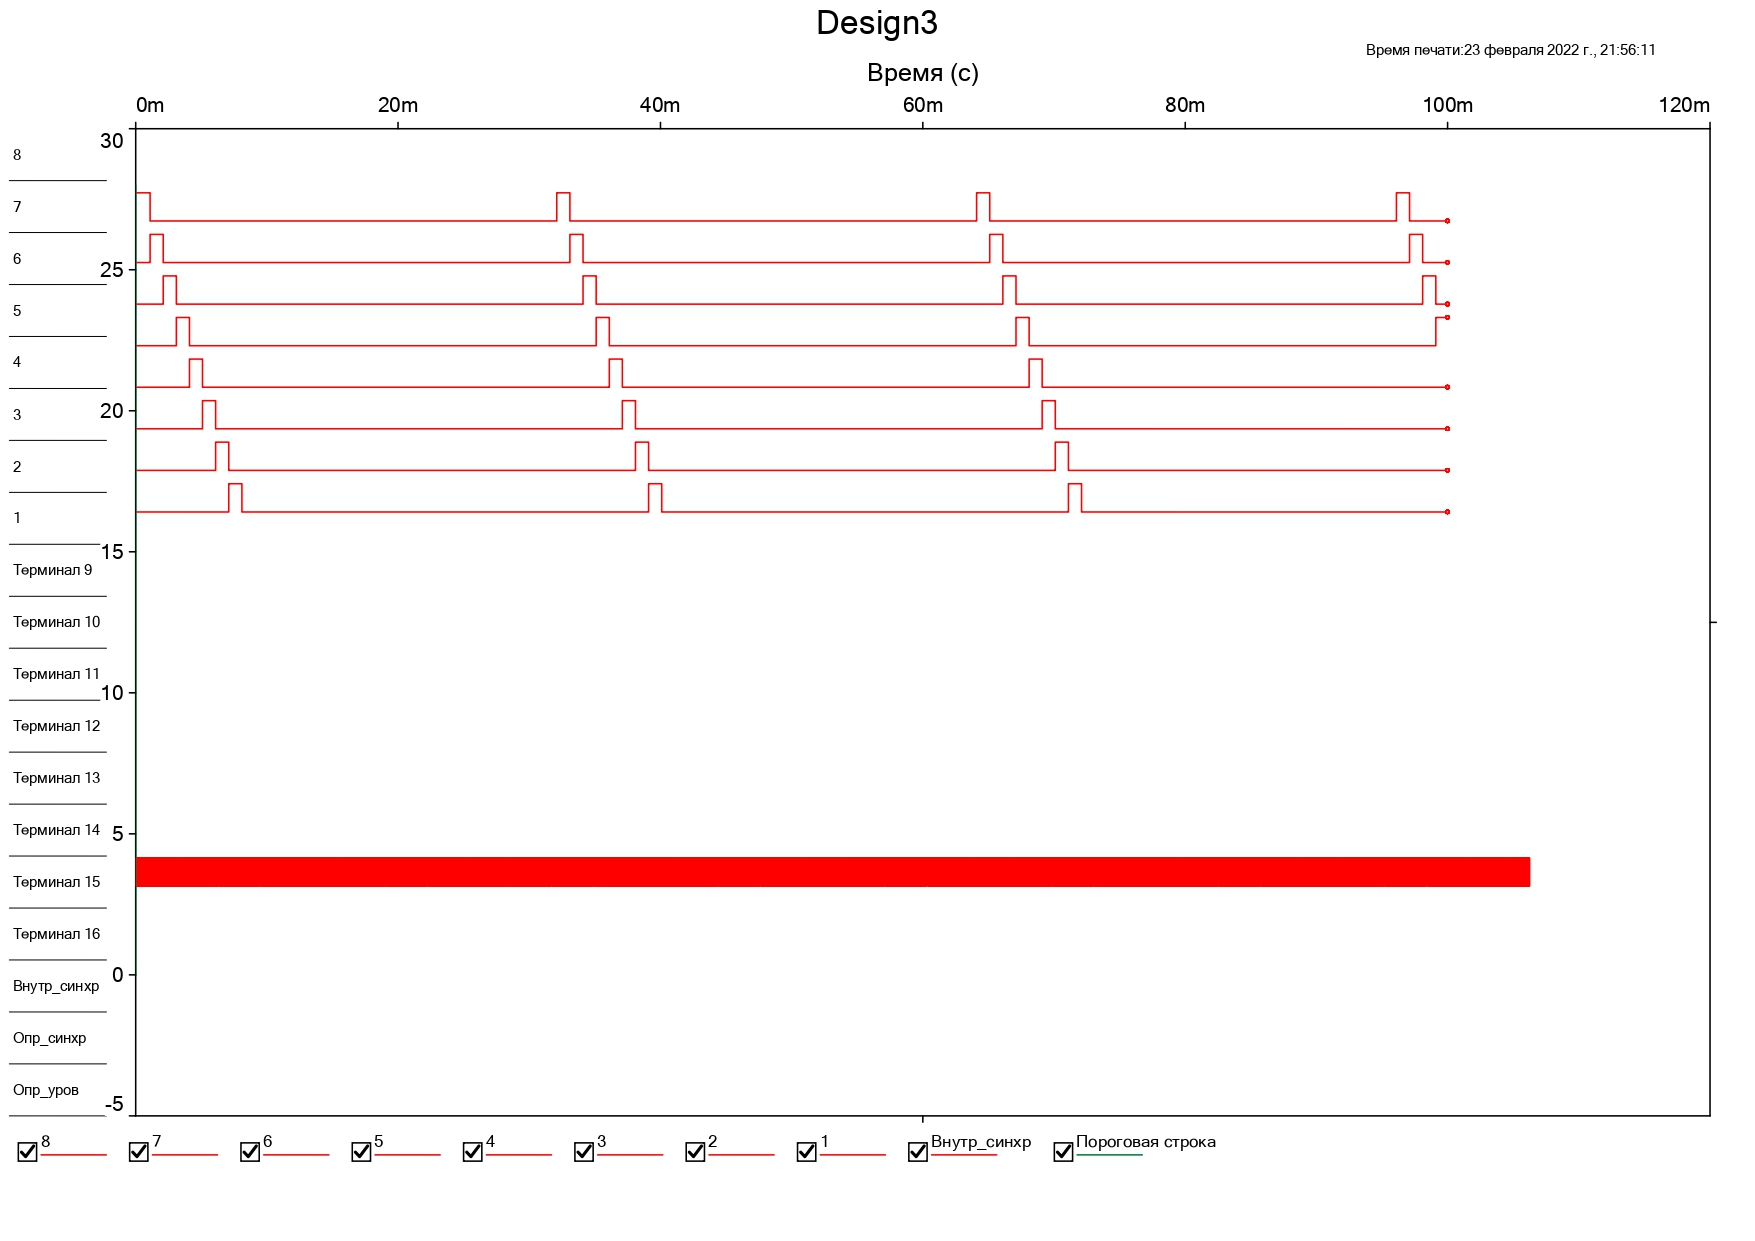
\includegraphics[width=1\linewidth]{3/graph.jpg}
\end{center}
\subsection{<<Логические элементы>>}
\begin{center}
    Таблица истинности
    \begin{table}[h!]
        \centering
        \begin{tabular}{|c|c|c|c|c|}
            \hline
            A & B & C & D & Result \\ \hline
            0 & 0 & 0 & 0 & 0      \\ \hline
            0 & 0 & 0 & 1 & 0      \\ \hline
            0 & 0 & 1 & 0 & 0      \\ \hline
            0 & 0 & 1 & 1 & 0      \\ \hline
            0 & 1 & 0 & 0 & 0      \\ \hline
            0 & 1 & 0 & 1 & 0      \\ \hline
            0 & 1 & 1 & 0 & 0      \\ \hline
            0 & 1 & 1 & 1 & 1      \\ \hline
            1 & 0 & 0 & 0 & 0      \\ \hline
            1 & 0 & 0 & 1 & 0      \\ \hline
            1 & 0 & 1 & 0 & 0      \\ \hline
            1 & 0 & 1 & 1 & 0      \\ \hline
            1 & 1 & 0 & 0 & 1      \\ \hline
            1 & 1 & 0 & 1 & 1      \\ \hline
            1 & 1 & 1 & 0 & 1      \\ \hline
            1 & 1 & 1 & 1 & 0      \\ \hline
        \end{tabular}
    \end{table}
\end{center}
\subsection{<<Исследование АЦП и ЦАП>>}
\begin{center}
    Осцилограмма
    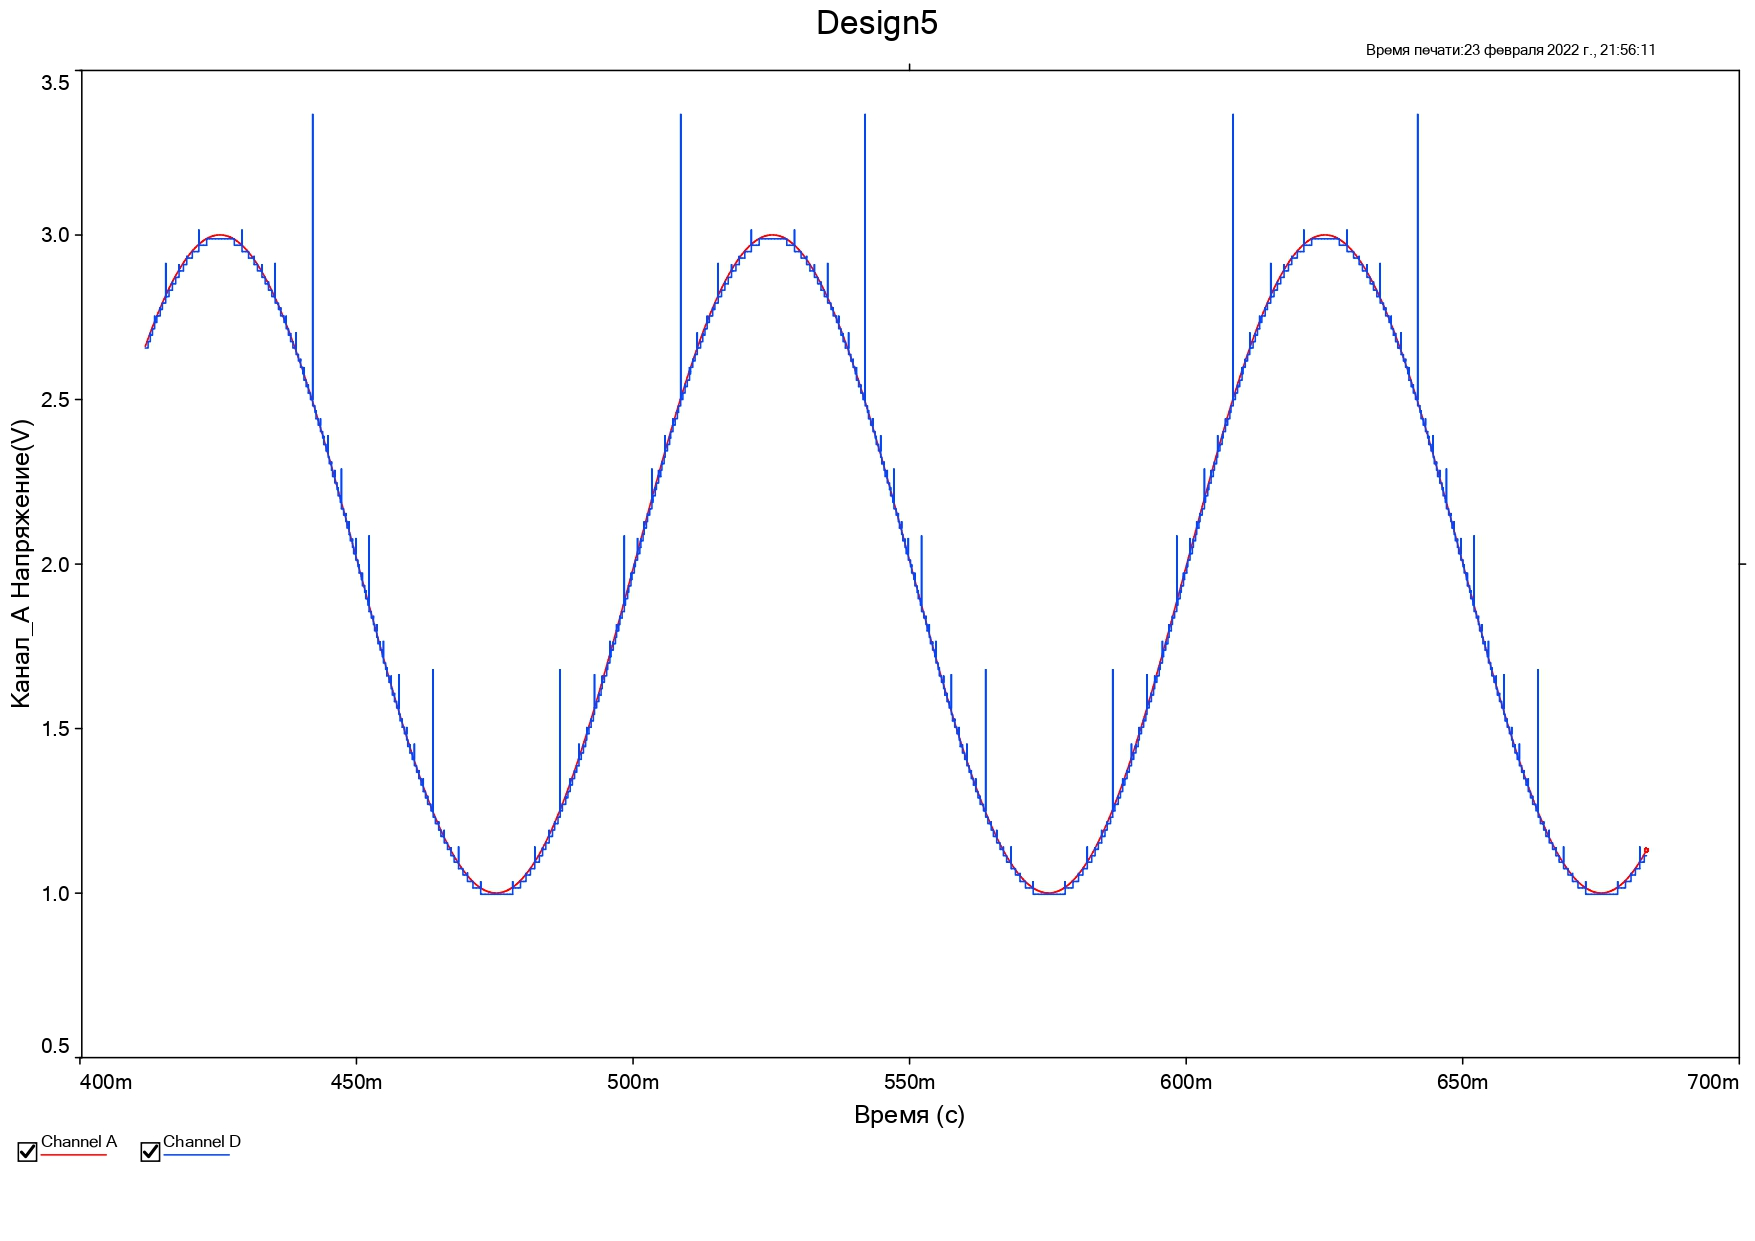
\includegraphics[width=1\linewidth]{5/graph.jpg}
\end{center}
\subsection{<<Исследование спектра сигналов>>}
Спектральный анализ
\begin{center}
    Ключ открыт
    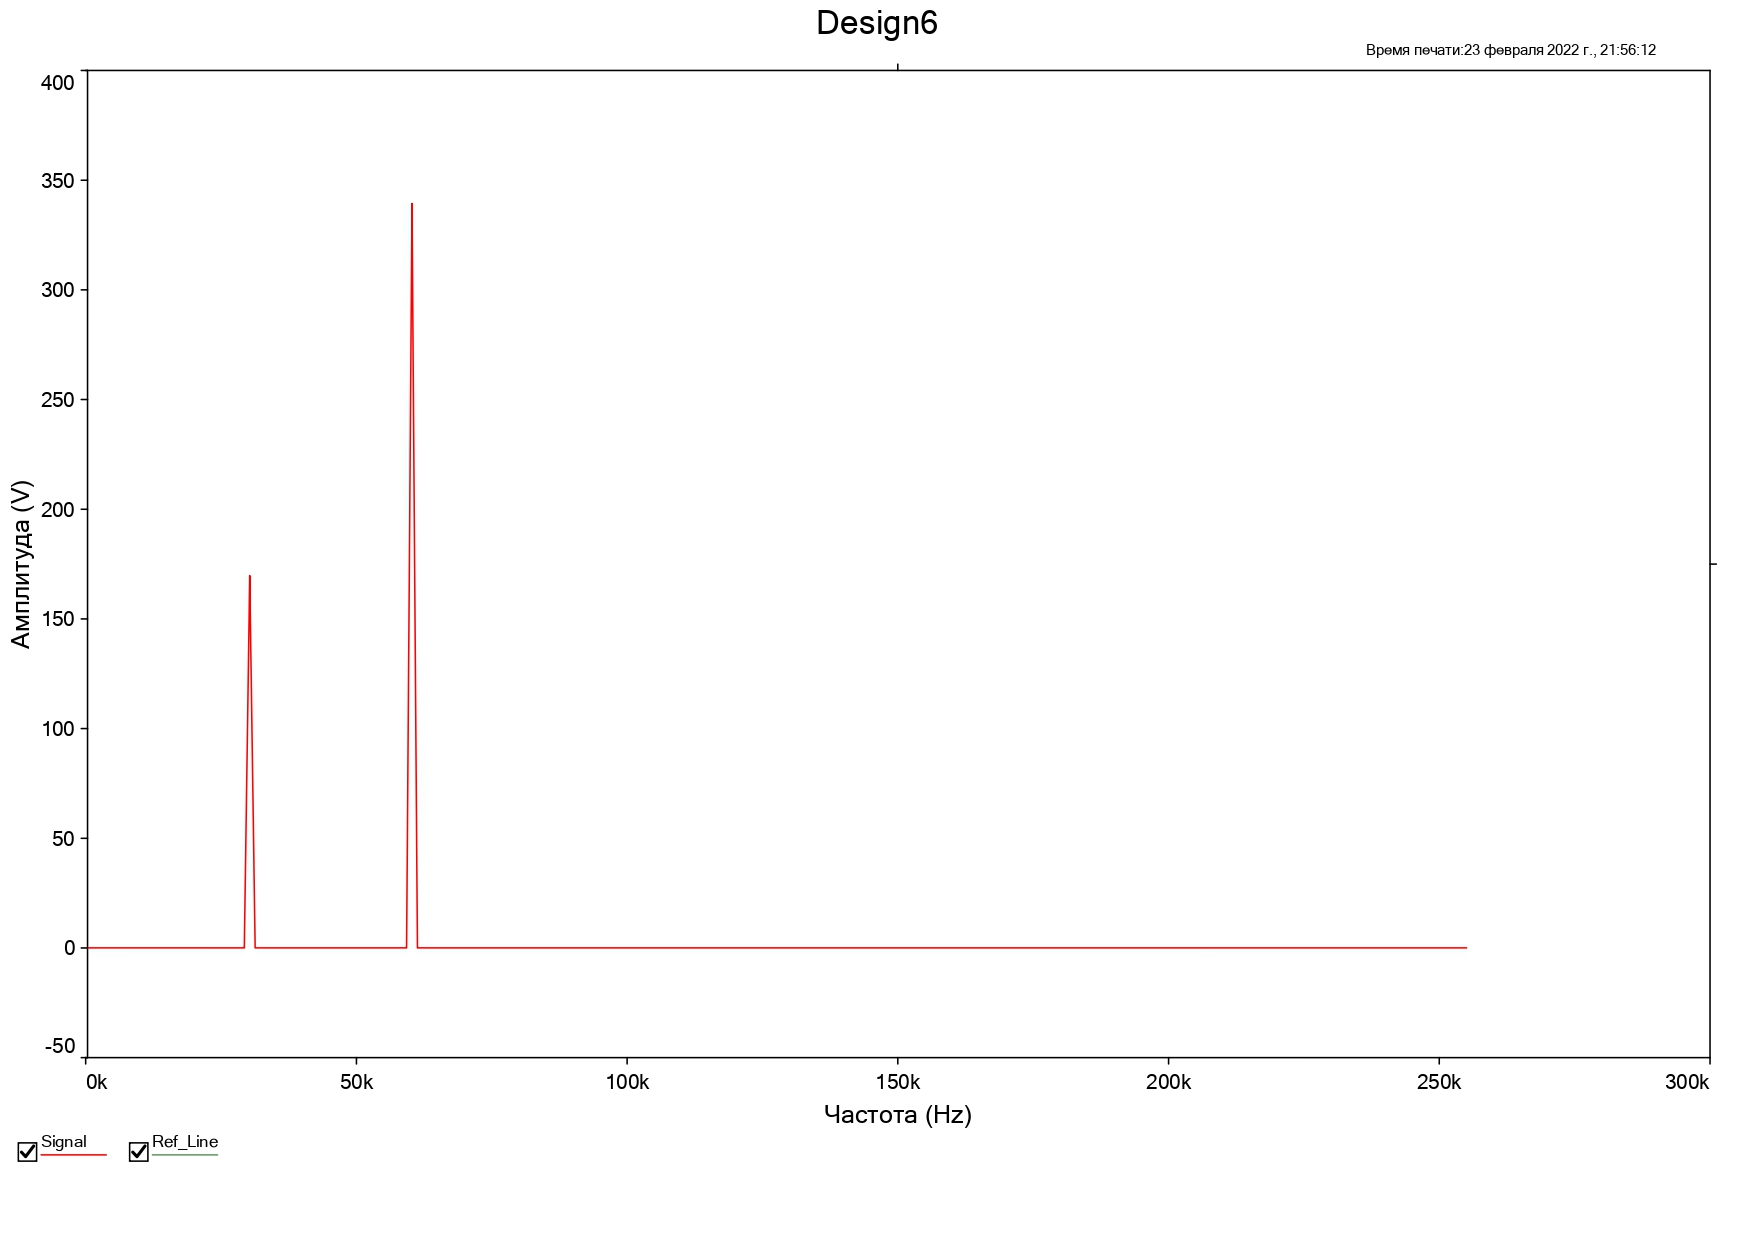
\includegraphics[width=1\linewidth]{6/graph_key_open.jpg}
    Ключ закрыт
    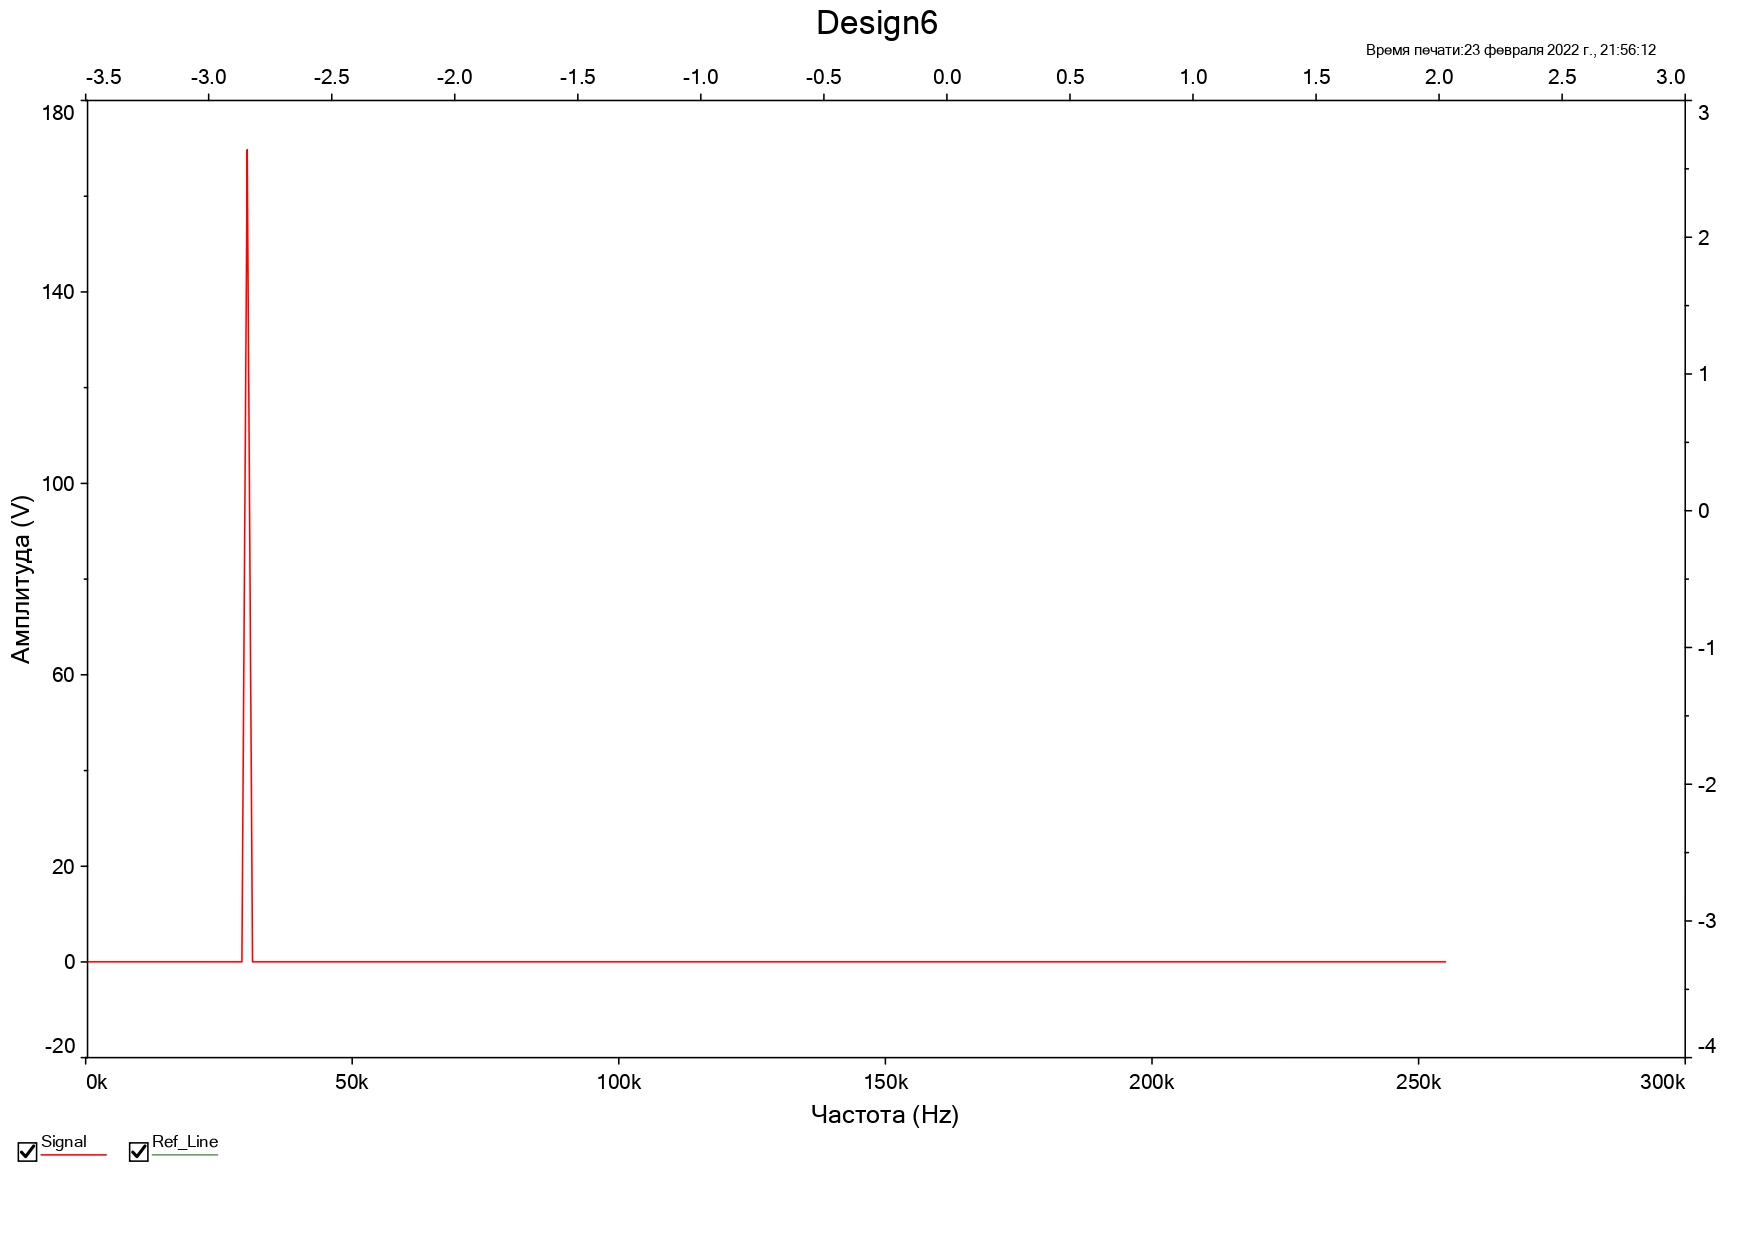
\includegraphics[width=1\linewidth]{6/graph_key_closed.jpg}
\end{center}
\textbf{Вывод:} в ходе выполнения лабораторной работы мы научились использовать возможности программы Multisim для изучения свойств сетей и систем передачи информации. На практике рассмотрели работу различных приборов для анализа схем аналоговой, цифровой и силовой электроники.
\end{document}

